\documentclass[11pt,a4paper]{article}

\usepackage[T1]{fontenc}
\usepackage[utf8]{inputenc}
\usepackage[a4paper,margin=27mm]{geometry}
\usepackage{amsmath,amssymb,amsthm,mathtools}
\usepackage{newpxtext,newpxmath}
\usepackage{microtype}
\usepackage{booktabs,tabularx,array}
\usepackage{enumitem}
\usepackage{graphicx}
\usepackage{xcolor}
\usepackage{titlesec}
\usepackage[authoryear,round]{natbib}
\usepackage[colorlinks=true,linkcolor=blue!45!black,
  citecolor=red!45!black,urlcolor=blue!45!black]{hyperref}

\definecolor{otblue}{HTML}{1F4E79}
\definecolor{otgray}{HTML}{F1F3F5}
\titleformat{\section}{\normalfont\Large\bfseries\color{otblue}}
  {\thesection}{.7em}{}
\titleformat{\subsection}{\normalfont\large\bfseries\color{otblue!80!black}}
  {\thesubsection}{.65em}{}
\titleformat{\paragraph}[runin]
  {\normalfont\bfseries\color{otblue!75!black}}{}{0pt}{}
\titlespacing*{\section}{0pt}{2.7ex plus .7ex minus .2ex}{1.1ex}
\titlespacing*{\subsection}{0pt}{2ex plus .5ex minus .2ex}{.75ex}
\titlespacing*{\paragraph}{0pt}{1.3ex plus .3ex minus .1ex}{.55em}

\newtheorem{theorem}{Theorem}[section]
\newtheorem{proposition}[theorem]{Proposition}
\newtheorem{corollary}[theorem]{Corollary}
\newtheorem{lemma}[theorem]{Lemma}
\theoremstyle{definition}
\newtheorem{definition}[theorem]{Definition}
\newtheorem{example}[theorem]{Example}
\theoremstyle{remark}
\newtheorem{remark}[theorem]{Remark}

\newcommand{\R}{\mathbb R}
\newcommand{\Pcal}{\mathcal P}
\newcommand{\Mcal}{\mathcal M}
\newcommand{\Lcal}{\mathcal L}
\newcommand{\Hcal}{\mathcal H}
\newcommand{\Id}{\operatorname{Id}}
\newcommand{\conv}{\operatorname{conv}}
\newcommand{\prox}{\operatorname{prox}}
\newcommand{\argmin}{\operatorname*{arg\,min}}
\newcommand{\dd}{\,\mathrm d}
\newcommand{\norm}[1]{\left\lVert #1\right\rVert}
\newcommand{\abs}[1]{\left\lvert #1\right\rvert}
\newcommand{\ip}[2]{\left\langle #1,#2\right\rangle}
\newcommand{\Perm}{\mathfrak P}

\hypersetup{
  pdftitle={The Monge Gap: Convexity, Rearrangements, and Kernel Regression},
  pdfauthor={Gabriel Peyre}
}

\title{The Monge Gap\\
  \large Convexity, rearrangements, and kernel regression}
\author{Gabriel Peyr\'e}
\date{July 2026}

\begin{document}
\maketitle

\begin{abstract}
The Monge gap of \citet{UsciddaCuturi2023} compares the cost of a candidate
map with the optimal transport cost between its input and output laws. Its
nonnegativity is automatic, but its convexity is not. We characterize the
smooth costs for which the gap is convex as a function of the map for every
source measure: up to terms depending on one marginal only, the cost must be
affine in the image variable. This class contains quadratic Mahalanobis costs
and reverse Bregman divergences; among smooth displacement costs
$h(x-y)$, it contains only quadratic functions, up to affine terms.

On the line, every convex displacement cost nevertheless has an explicit
quantile formula. For a strictly convex cost its gap vanishes exactly on
increasing maps, but the resulting monotonicity penalty is generally
nonconvex. The quadratic case is exceptional: the gap is the deficit in the
Hardy--Littlewood rearrangement inequality, or equivalently the support
function of a translated permutahedron. This identifies its precise relation
to isotonic regression and turns Monge-gap-regularized kernel regression into
a finite convex program. For equally spaced inputs, the regularizer is a sum
of pairwise hinge losses over all order inversions, yielding a standard
quadratic program and a simple numerical experiment.
\end{abstract}

\section{The exact Monge gap}

The Monge gap separates marginal fitting from transport optimality. A fitting
loss can require that a learned map reaches a prescribed target; the gap asks
whether that map transports its own output law as cheaply as possible.

\subsection{Definition and self-coupling representation}

Let $\mathcal X$ be a standard Borel space, let $\mathcal Y\subset\R^m$, let
$\rho\in\Pcal(\mathcal X)$, and let $T:\mathcal X\to\mathcal Y$ be
measurable. For a lower-semicontinuous cost
$c:\mathcal X\times\mathcal Y\to\R\cup\{+\infty\}$, write
\[
  \Lcal_c(\alpha,\beta)
  :=\inf_{\pi\in\Pi(\alpha,\beta)}\int c(x,y)\,\dd\pi(x,y)
\]
whenever the relevant integrals are well defined.

\begin{definition}[Monge gap \citealp{UsciddaCuturi2023}]
The $c$-Monge gap of $T$ relative to $\rho$ is
\begin{equation}\label{eq:general-monge-gap}
  \Mcal_\rho^c(T)
  :=\int c(x,T(x))\,\dd\rho(x)
    -\Lcal_c(\rho,T_\#\rho).
\end{equation}
\end{definition}

The first term is the cost of the graph coupling
$\pi_T=(\Id,T)_\#\rho$; the second is the smallest cost among all couplings
with the same marginals. Consequently,
\begin{equation}\label{eq:gap-zero-optimal}
  \Mcal_\rho^c(T)\geq0,
  \qquad
  \Mcal_\rho^c(T)=0
  \quad\Longleftrightarrow\quad
  (\Id,T)_\#\rho\text{ is optimal}.
\end{equation}

The dependence of the second marginal on $T$ obscures the geometry of the
functional. Lifting every coupling back to two copies of the source removes
this difficulty.

\begin{lemma}[Lifting through a map]\label{lem:coupling-lift}
For every $\pi\in\Pi(\rho,T_\#\rho)$, there exists
$\eta\in\Pi(\rho,\rho)$ such that the map $(x,z)\mapsto(x,T(z))$ pushes
$\eta$ to $\pi$.
\end{lemma}

\begin{proof}
Disintegrate $\rho$ along $T$ as
$\rho(\dd z)=\int\rho_y(\dd z)(T_\#\rho)(\dd y)$, where $\rho_y$ is
concentrated on $T^{-1}(y)$, and disintegrate
$\pi(\dd x,\dd y)=\pi_y(\dd x)(T_\#\rho)(\dd y)$. Then
\[
  \eta(\dd x,\dd z)
  :=\int \pi_y(\dd x)\rho_y(\dd z)(T_\#\rho)(\dd y)
\]
has both marginals equal to $\rho$, and $T(z)=y$ almost surely.
\end{proof}

\begin{proposition}[General self-coupling formula]\label{prop:general-self-coupling}
Assume that all terms below are finite. Then
\begin{align}
  \Lcal_c(\rho,T_\#\rho)
  &=\inf_{\eta\in\Pi(\rho,\rho)}
      \int c(x,T(z))\,\dd\eta(x,z),\label{eq:lifted-transport}\\
  \Mcal_\rho^c(T)
  &=\sup_{\eta\in\Pi(\rho,\rho)}
      \int\bigl[c(x,T(x))-c(x,T(z))\bigr]\,\dd\eta(x,z).
      \label{eq:general-self-gap}
\end{align}
\end{proposition}

\begin{proof}
Every self-coupling $\eta$ induces an admissible coupling by
$(x,z)\mapsto(x,T(z))$, while Lemma~\ref{lem:coupling-lift} shows that every
admissible coupling has such a lift. This proves
\eqref{eq:lifted-transport}; subtracting it from the graph cost gives
\eqref{eq:general-self-gap}.
\end{proof}

Formula~\eqref{eq:general-self-gap} is always an optimality-gap
representation. It is not generally a supremum of convex, let alone linear,
functions of $T$. The next section identifies exactly when this cancellation
does occur for smooth costs.

\section{Which costs give a convex Monge gap?}

Convexity for one fixed source may result from accidental symmetries. A useful
cost-level statement should instead hold for every source measure. Under mild
smoothness, this universal requirement has a sharp answer.

\subsection{Affine differences characterize universal convexity}

Call $c$ an \emph{affine-difference cost} if, for every $x_0,x_1$, the map
$y\mapsto c(x_0,y)-c(x_1,y)$ is affine. Equivalently, after choosing an
origin in $\mathcal Y$, it can be written
\begin{equation}\label{eq:affine-difference-cost}
  c(x,y)=a(x)+b(y)-\ip{A(x)}{y}
\end{equation}
for some scalar functions $a,b$ and a map $A:\mathcal X\to\R^m$. The terms
$a(x)$ and $b(y)$ depend on one marginal only and disappear from the gap.

\begin{theorem}[Smooth convexity characterization]\label{thm:cost-convexity-characterization}
Let $\mathcal Y\subset\R^m$ be open and convex, and assume that
$c(x,\cdot)\in C^2(\mathcal Y)$ for every $x$. The following statements are
equivalent.
\begin{enumerate}[label=(\roman*)]
  \item For every finitely supported source $\rho$, the map
    $T\mapsto\Mcal_\rho^c(T)$ is convex on its finite-dimensional space of
    values.
  \item The same convexity holds for every equal-weight two-point source.
  \item Every difference $c(x_0,\cdot)-c(x_1,\cdot)$ is affine.
  \item The cost has the affine-difference form
    \eqref{eq:affine-difference-cost}.
\end{enumerate}
For such a cost,
\begin{equation}\label{eq:affine-difference-gap}
  \Mcal_\rho^c(T)
  =\sup_{\eta\in\Pi(\rho,\rho)}
    \int\ip{A(x)}{T(z)-T(x)}\,\dd\eta(x,z),
\end{equation}
so the gap is convex. When $\mathcal Y=\R^m$ (or the admissible map class is
stable under nonnegative scaling), it is also positively homogeneous in $T$.
\end{theorem}

\begin{proof}
Clearly (i) implies (ii). Fix $x_0,x_1$ and set
$\rho=\tfrac12(\delta_{x_0}+\delta_{x_1})$. A map is determined by
$u=T(x_0)$ and $v=T(x_1)$. The two extreme self-couplings are the identity
and the transposition, hence
\begin{equation}\label{eq:two-point-general-gap}
  \Mcal_\rho^c(T)
  =\frac12\bigl[g(u)-g(v)\bigr]_+,
  \qquad
  g(y):=c(x_0,y)-c(x_1,y).
\end{equation}
Suppose this function is convex in $(u,v)$. On the open set $g(u)>g(v)$,
its Hessian is
\[
  \frac12
  \begin{pmatrix}
    \nabla^2g(u)&0\\[1mm]0&-\nabla^2g(v)
  \end{pmatrix},
\]
which must be positive semidefinite. Thus $\nabla^2g(u)\succeq0$ at every
point whose value exceeds another value, and $\nabla^2g(v)\preceq0$ at every
point whose value is below another one. A point that is neither a global
minimum nor a global maximum satisfies both inequalities. At a global
minimum or maximum, the missing inequality follows from the ordinary
second-order extremum condition. Hence $\nabla^2g=0$ everywhere; $g$ is
affine. This proves (ii)$\Rightarrow$(iii).

Choose a fixed $\bar x$. By (iii),
$c(x,y)-c(\bar x,y)=a(x)-\ip{A(x)}{y}$ for suitable $a,A$; taking
$b(y)=c(\bar x,y)$ gives (iv). Finally, insert
\eqref{eq:affine-difference-cost} into
\eqref{eq:general-self-gap}. Since both marginals of $\eta$ equal $\rho$,
the integrals of $b(T(x))$ and $b(T(z))$ cancel, which gives
\eqref{eq:affine-difference-gap}. It is a supremum of linear functionals of
$T$, proving (i) and the final claim.
\end{proof}

This theorem is a universal statement: a particular pair $(c,\rho)$ may
still produce a convex gap outside this class. Conversely, the two-point
formula~\eqref{eq:two-point-general-gap} is a cheap diagnostic that disproves
universal convexity.

\subsection{Examples and a counterexample}

\paragraph{Quadratic and Mahalanobis costs.}
For $Q\succeq0$,
\[
  c_Q(x,y)=\frac12(x-y)^\top Q(x-y)
\]
has the form~\eqref{eq:affine-difference-cost} with $A(x)=Qx$. The usual
quadratic cost corresponds to $Q=\Id$.

\paragraph{Reverse Bregman divergences.}
If $F$ is differentiable and convex, then
\[
  D_F(y,x):=F(y)-F(x)-\ip{\nabla F(x)}{y-x}
\]
is also an affine-difference cost, with $A(x)=\nabla F(x)$. Thus a genuinely
nonquadratic cost can have a convex Monge gap. The orientation matters:
$D_F(x,y)$ is generally nonlinear in the second argument in a way that does
not cancel.

\begin{corollary}[Smooth displacement costs]\label{cor:displacement-classification}
Let $c(x,y)=h(x-y)$ with $h\in C^2(\R^d)$. The Monge gap is convex in $T$ for
every finitely supported source if and only if
\begin{equation}\label{eq:quadratic-displacement}
  h(z)=\frac12z^\top Qz+r^\top z+s
\end{equation}
for a symmetric matrix $Q$. If $h$ is convex, then necessarily $Q\succeq0$.
The affine terms do not affect the gap.
\end{corollary}

\begin{proof}
Theorem~\ref{thm:cost-convexity-characterization} requires
$\nabla_y^2c(x,y)=\nabla^2h(x-y)$ to be independent of $x$. Hence
$\nabla^2h$ is constant, which gives~\eqref{eq:quadratic-displacement}.
The converse follows from the Mahalanobis example.
\end{proof}

\begin{example}[A convex cost with a nonconvex gap]\label{ex:quartic-counterexample}
Take $c(x,y)=(x-y)^4$ on the line and
$\rho=\tfrac12(\delta_{-1}+\delta_1)$. Let $T_-$, $T_0$, and $T_+$ take the
following values at $(-1,1)$:
\[
  T_-=(-3/2,-2),\qquad T_0=(-1,-2),\qquad T_+=(-1/2,-2).
\]
Then $T_0=(T_-+T_+)/2$, while direct evaluation of the two possible
assignments gives
\[
  \Mcal_\rho^c(T_-)=20.5,qquad
  \Mcal_\rho^c(T_0)=32,qquad
  \Mcal_\rho^c(T_+)=37.5.
\]
Thus $32>(20.5+37.5)/2=29$: even a smooth strictly convex displacement cost
need not yield a convex Monge gap.
\end{example}

\subsection{The quadratic support function}

For $c_2(x,y)=\tfrac12\norm{x-y}^2$ and
$\rho\in\Pcal_2(\R^d)$, formula~\eqref{eq:affine-difference-gap} becomes
\begin{equation}\label{eq:quadratic-support-form}
  \Mcal_\rho^2(T)
  =\sup_{\eta\in\Pi(\rho,\rho)}
  \left\{
    \int x\mathbin{\cdot}T(z)\,\dd\eta(x,z)
    -\int x\mathbin{\cdot}T(x)\,\dd\rho(x)
  \right\}.
\end{equation}
It follows immediately that $\Mcal_\rho^2$ is convex, nonnegative,
subadditive, and positively homogeneous on $L^2(\rho;\R^d)$. Under Brenier's
assumptions, its zero set has the expected geometric interpretation.

\begin{proposition}[Zero set of the quadratic gap]\label{prop:quadratic-zero-set}
If $\rho$ is absolutely continuous with respect to Lebesgue measure, then
\[
  \Mcal_\rho^2(T)=0
  \quad\Longleftrightarrow\quad
  T=\nabla\varphi\quad\rho\text{-a.e. for some convex }\varphi.
\]
For a finitely supported source, zero gap is equivalent to cyclical
monotonicity of the pairs $(x_i,T(x_i))$, or to
$T(x_i)\in\partial\varphi(x_i)$ for a convex $\varphi$.
\end{proposition}

\begin{proof}
By~\eqref{eq:gap-zero-optimal}, zero gap means that the graph coupling is
quadratically optimal. Brenier's theorem gives the first statement
\citep{Brenier1991,Villani2009}; Rockafellar's theorem gives the finite
cyclical-monotonicity statement \citep{Rockafellar1966}.
\end{proof}

Convexity is in the free map values, not necessarily in a parametrization. If
$T=T_\theta$ is a neural network, the composition
$\theta\mapsto\Mcal_\rho^2(T_\theta)$ is generally nonconvex.

\section{One-dimensional rearrangement formulas}

The line offers an explicit formula for every convex displacement cost. This
is enough to recognize monotone maps, but not enough to make the penalty
convex: Example~\ref{ex:quartic-counterexample} already occurs in one
dimension.

\subsection{General convex displacement costs}

For a probability measure $\alpha$ on $\R$, denote its cumulative function by
$F_\alpha(x)=\alpha(( -\infty,x])$ and its generalized quantile by
\[
  Q_\alpha(s):=\inf\{x:F_\alpha(x)\geq s\},\qquad s\in(0,1).
\]

\begin{proposition}[Closed one-dimensional Monge-gap formula]
\label{prop:one-dimensional-gap}
Let $c(x,y)=h(x-y)$ with $h:\R\to\R$ convex, let $\rho\in\Pcal(\R)$, and set
$\beta=T_\#\rho$. Under the corresponding integrability assumptions,
\begin{equation}\label{eq:general-1d-gap}
  \Mcal_\rho^h(T)
  =\int h(x-T(x))\,\dd\rho(x)
   -\int_0^1 h\bigl(Q_\rho(s)-Q_\beta(s)\bigr)\,\dd s.
\end{equation}
If $\rho$ is atomless, define the increasing rearrangement of $T$ by
\begin{equation}\label{eq:increasing-rearrangement}
  T^\uparrow(x):=Q_\beta(F_\rho(x)).
\end{equation}
Then $(T^\uparrow)_\#\rho=\beta$ and
\begin{equation}\label{eq:rearrangement-gap}
  \Mcal_\rho^h(T)
  =\int\bigl[h(x-T(x))-h(x-T^\uparrow(x))\bigr]\,\dd\rho(x).
\end{equation}
If $h$ is strictly convex, the gap vanishes exactly when $T$ has a
nondecreasing representative $\rho$-almost everywhere. For merely convex
$h$, monotonicity is sufficient but need not be necessary.
\end{proposition}

\begin{proof}
For $x<x'$ and $y<y'$, convexity of $h$ gives the Monge inequality
\[
  h(x-y)+h(x'-y')\leq h(x-y')+h(x'-y).
\]
Indeed, the increment $r\mapsto h(r+y'-y)-h(r)$ is nondecreasing. Repeatedly
uncrossing inverted pairs therefore shows that the quantile coupling
$(Q_\rho,Q_\beta)_\#\mathcal U(0,1)$ is optimal. This proves
\eqref{eq:general-1d-gap}. If $\rho$ is atomless, $F_\rho(X)$ is uniform for
$X\sim\rho$, so~\eqref{eq:increasing-rearrangement} realizes the quantile
coupling as a map and gives~\eqref{eq:rearrangement-gap}. Strict convexity
makes every genuine crossing strictly more expensive, yielding the final
characterization.
\end{proof}

For an equal-weight empirical source with
$x_1<\cdots<x_n$, write $t_i=T(x_i)$ and let
$t_{(1)}\leq\cdots\leq t_{(n)}$ be their order statistics. Then
\begin{equation}\label{eq:empirical-general-h-gap}
  \Mcal_{\widehat\rho}^h(t)
  =\frac1n\sum_{i=1}^n
    \bigl[h(x_i-t_i)-h(x_i-t_{(i)})\bigr].
\end{equation}
Thus the gap is evaluated by one sort, in $O(n\log n)$ time. This is an exact
penalty for violations of increasing order when $h$ is strictly convex, but
Corollary~\ref{cor:displacement-classification} shows that it is generally
nonconvex in $t$ unless $h$ is quadratic up to affine terms.

\subsection{Quadratic cost, covariance deficit, and permutahedra}

For $h(r)=r^2/2$, all target second moments cancel. Proposition
\ref{prop:one-dimensional-gap} simplifies to
\begin{equation}\label{eq:quadratic-covariance-gap}
  \Mcal_\rho^2(T)
  =\int_0^1 Q_\rho(s)Q_{T_\#\rho}(s)\,\dd s
    -\int xT(x)\,\dd\rho(x).
\end{equation}
The first term is the largest possible cross-moment, or covariance, among all
couplings of $\rho$ and $T_\#\rho$. Hence the one-dimensional quadratic Monge
gap is precisely the deficit in the Hardy--Littlewood rearrangement inequality
\citep{HardyLittlewoodPolya1952}. ``Rearrangement deficit'' or
``comonotonicity deficit'' describes this quantity accurately; there does not
appear to be a separate canonical name for this exact functional.

For empirical data, let $x=(x_1,\ldots,x_n)^\top$ and
$t=(t_1,\ldots,t_n)^\top$, with $x_1<\cdots<x_n$. Define the permutahedron
\[
  \Perm(x):=\conv\{P_\sigma x:\sigma\in\mathfrak S_n\}
\]
and the support function $\sigma_C(t):=\sup_{q\in C}q^\top t$. The
rearrangement inequality gives
\begin{equation}\label{eq:permutahedron-gap}
  \Mcal_{\widehat\rho}^2(t)
  =\frac1n\bigl(x^\top t^\uparrow-x^\top t\bigr)
  =\frac1n\bigl(\sigma_{\Perm(x)}(t)-x^\top t\bigr)
  =\sigma_{D_x}(t),
  \qquad
  D_x:=\frac{\Perm(x)-x}{n}.
\end{equation}
This proves convexity directly. If the entries of $t$ are distinct, a
subgradient is $(q^\star-x)/n$, where $q^\star$ permutes the entries of $x$
into the rank order of $t$. Moreover,
\begin{equation}\label{eq:zero-monotone-cone}
  \Mcal_{\widehat\rho}^2(t)=0
  \quad\Longleftrightarrow\quad
  t_1\leq\cdots\leq t_n.
\end{equation}

There is an especially transparent formula on a uniform grid.

\begin{proposition}[Pairwise inversion formula]\label{prop:pairwise-hinge}
If $x_i=x_1+(i-1)\Delta$ with $\Delta>0$, then
\begin{equation}\label{eq:pairwise-hinge}
  \Mcal_{\widehat\rho}^2(t)
  =\frac{\Delta}{n}
    \sum_{1\leq i<j\leq n}(t_i-t_j)_+.
\end{equation}
For $n=2$, this reduces to
$\Mcal_{\widehat\rho}^2(t)=\tfrac{x_2-x_1}{2}(t_1-t_2)_+$.
\end{proposition}

\begin{proof}
Bubble-sorting $t$ exchanges each inverted pair exactly once. Swapping two
adjacent inverted values $u>v$ increases $x^\top t$ by
$\Delta(u-v)$. Summing these increments over all inversions and dividing by
$n$ gives~\eqref{eq:pairwise-hinge}.
\end{proof}

Formula~\eqref{eq:pairwise-hinge} is the zero-margin pairwise ranking hinge
summed over every inversion. It is therefore a polyhedral exact penalty for
the monotone cone.

\subsection{What is the relation with isotonic regression?}

Classical least-squares isotonic regression computes the metric projection
\begin{equation}\label{eq:isotonic-regression}
  \Pi_{\mathcal C}(z)
  :=\argmin_{t_1\leq\cdots\leq t_n}\frac12\norm{t-z}^2,
  \qquad
  \mathcal C:=\{t:t_1\leq\cdots\leq t_n\}.
\end{equation}
The Monge gap and isotonic regression have the same target set
$\mathcal C$, but they are not the same operation:
\begin{itemize}
  \item rearrangement sorts the existing values and preserves their empirical
    distribution;
  \item isotonic regression moves and pools values to minimize a metric
    fitting error;
  \item the Monge gap measures the improvement obtained by rearranging the
    graph coupling, rather than the distance from $t$ to $\mathcal C$.
\end{itemize}

The precise computational link goes through the permutahedron. Since
$\Mcal_{\widehat\rho}^2=\sigma_{D_x}$, the proximal map satisfies
\begin{equation}\label{eq:gap-prox-permutahedron}
  \prox_{\tau\Mcal_{\widehat\rho}^2}(z)
  =z-\tau\Pi_{D_x}(z/\tau)
  =z-\Pi_{\tau D_x}(z).
\end{equation}
Projection onto a permutahedron reduces, after sorting, to isotonic
optimization and can be solved by pool-adjacent-violators-type algorithms
\citep{LimWright2016}. Thus isotonic regression is an algorithmic primitive
for proximal computations with the quadratic Monge gap, even though the gap
itself is not an isotonic projection loss.

\section{Kernel regression with a Monge-gap penalty}

The preceding formulas make the proposed experiment tractable without any
transport solver. Consider scalar regression data
$x_1<\cdots<x_n$ and $y_1,\ldots,y_n$, and a scalar RKHS $\Hcal_k$. For the
quadratic Monge gap relative to
$\widehat\rho=n^{-1}\sum_i\delta_{x_i}$, define
\begin{equation}\label{eq:rkhs-monge-problem}
  \min_{T\in\Hcal_k}
  \left\{
    \sum_{i=1}^n\abs{T(x_i)-y_i}^2
    +\lambda\norm{T}_{\Hcal_k}^2
    +\gamma\Mcal_{\widehat\rho}^2(T)
  \right\},
  \qquad \lambda>0,\quad\gamma\geq0.
\end{equation}

\subsection{Convexity and the kernel reduction}

All three terms in~\eqref{eq:rkhs-monge-problem} are convex in $T$, and the
RKHS term is strictly convex. Hence the problem has at most one minimizer; the
usual coercivity and lower-semicontinuity assumptions give existence. More
importantly, the kernel trick is exact.

\begin{proposition}[Representer theorem and finite convex program]
\label{prop:rkhs-representer}
Every minimizer of~\eqref{eq:rkhs-monge-problem} has the form
\begin{equation}\label{eq:representer}
  T(\cdot)=\sum_{j=1}^n a_j k(x_j,\cdot).
\end{equation}
Let $K_{ij}=k(x_i,x_j)$, $a=(a_j)_j$, and $y=(y_i)_i$. The coefficients solve
the finite convex problem
\begin{equation}\label{eq:kernel-finite-program}
  \min_{a\in\R^n}
  \left\{
    \norm{Ka-y}^2+\lambda a^\top Ka
    +\frac{\gamma}{n}
      \bigl[\sigma_{\Perm(x)}(Ka)-x^\top Ka\bigr]
  \right\}.
\end{equation}
If $K$ is positive definite, this program has a unique coefficient vector.
\end{proposition}

\begin{proof}
Decompose any $T\in\Hcal_k$ into its orthogonal projection onto
$\operatorname{span}\{k(x_i,\cdot)\}_{i=1}^n$ and an orthogonal remainder.
The remainder vanishes at every $x_i$, so it changes neither the data term nor
the Monge gap, while it strictly increases the squared RKHS norm unless it is
zero. This proves~\eqref{eq:representer}, the classical representer argument
\citep{KimeldorfWahba1971,ScholkopfHerbrichSmola2001}. The identities
$T(x_i)=(Ka)_i$ and $\norm{T}_{\Hcal_k}^2=a^\top Ka$, together with
\eqref{eq:permutahedron-gap}, give~\eqref{eq:kernel-finite-program}. Convexity
follows because a support function composed with a linear map is convex.
\end{proof}

The support function is evaluated by sorting $Ka$, in $O(n\log n)$ time. A
subgradient is obtained from the same ranks, so bundle, subgradient, and
proximal methods require no $n\times n$ transport optimization.

\paragraph{Uniform-grid quadratic program.}
If the inputs are equally spaced with step $\Delta$, introduce variables
$\xi_{ij}$ for $i<j$. Proposition~\ref{prop:pairwise-hinge} turns
\eqref{eq:kernel-finite-program} into
\begin{equation}\label{eq:kernel-qp}
\begin{aligned}
  \min_{a,\xi}\quad &
    \norm{Ka-y}^2+\lambda a^\top Ka
    +\frac{\gamma\Delta}{n}\sum_{i<j}\xi_{ij},\\
  \text{subject to}\quad &
    \xi_{ij}\geq(Ka)_i-(Ka)_j,qquad
    \xi_{ij}\geq0\qquad(i<j).
\end{aligned}
\end{equation}
This is a convex quadratic program with $n$ kernel coefficients and
$n(n-1)/2$ scalar slack variables. The quadratic number of slacks is suitable
for a moderate experiment; sorting-oracle methods are preferable at large
$n$. Since the penalty is polyhedral and vanishes exactly on the monotone
cone, standard exact-penalty theory also implies that, under the usual
constraint qualification, a finite sufficiently large $\gamma$ recovers the
hard monotone RKHS fit.

\paragraph{Dual projection viewpoint.}
If $K$ is positive definite, use the fitted values $t=Ka$ and set
\[
  Q:=I+\lambda K^{-1},
  \qquad D_x:=\frac{\Perm(x)-x}{n}.
\]
For $\gamma>0$, Fenchel duality gives
\begin{equation}\label{eq:kernel-dual-projection}
  d^\star
  =\argmin_{d\in D_x}
     \left(d-\frac{2y}{\gamma}\right)^\top
       Q^{-1}
     \left(d-\frac{2y}{\gamma}\right),
  \qquad
  t^\star=Q^{-1}\left(y-\frac\gamma2d^\star\right).
\end{equation}
Indeed, write $\sigma_{D_x}(t)=\max_{d\in D_x}d^\top t$ and minimize the
resulting strongly convex quadratic in $t$. Equation
\eqref{eq:kernel-dual-projection} is a projection onto a translated
permutahedron in the kernel-induced metric $Q^{-1}$. When that metric is
diagonal, this is a separable isotonic optimization problem. For a general
kernel, $Q^{-1}$ is dense, so ordinary pool-adjacent violators is not by
itself a complete solver; the quadratic program~\eqref{eq:kernel-qp} or a
general metric-projection method is still needed.

\subsection{A numerical feasibility experiment}

Figure~\ref{fig:kernel-monge-regression} solves~\eqref{eq:kernel-qp} for
$55$ equally spaced inputs, a Gaussian kernel, and several values of
$\gamma$. The observations deliberately follow a smooth but nonmonotone
trend. Increasing $\gamma$ progressively removes order inversions; at the
largest displayed value the solution agrees numerically with the hard
monotone RKHS fit. The experiment is generated by
\texttt{kernel\_monge\_regression.py} in this directory.

\begin{figure}[ht]
  \centering
  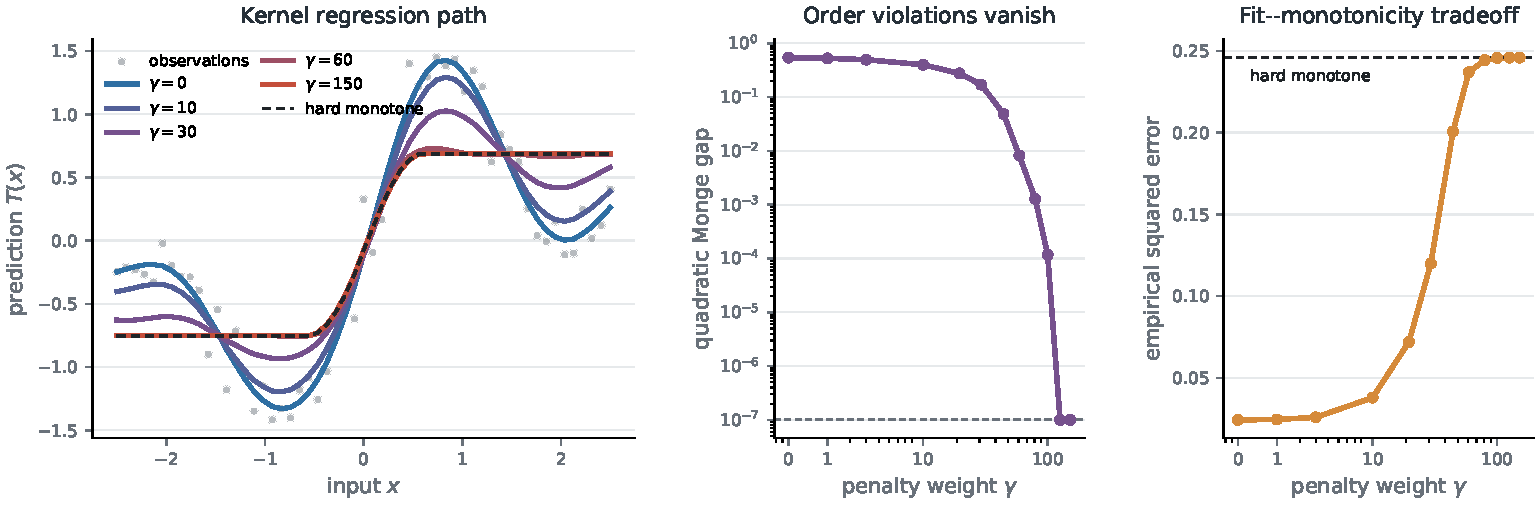
\includegraphics[width=\textwidth]{kernel_monge_regression.pdf}
  \caption{\emph{Monge-gap-regularized kernel regression is a convex
  monotonicity path.} Left: Gaussian-RKHS fits evolve from an unconstrained
  smooth regressor (blue) to the hard monotone fit (red) as $\gamma$
  increases. Center: the exact empirical quadratic Monge gap decreases to
  numerical zero. Right: the data error increases as monotonicity is imposed;
  the dashed line marks the hard monotone solution.}
  \label{fig:kernel-monge-regression}
\end{figure}

This confirms feasibility, but also exposes the modeling choice: the penalty
does not merely smooth the regression curve. It favors maps whose sampled
graph is optimal for quadratic transport, which on the line means increasing
order.

\subsection{What changes for a general convex \texorpdfstring{$h$}{h}?}

The representer argument does not require a quadratic cost. For any empirical
loss that depends on $T$ only through $(T(x_i))_i$, a minimizer still has the
form~\eqref{eq:representer}. With a convex displacement cost $h$, the finite
objective becomes
\begin{equation}\label{eq:kernel-general-h}
  \norm{Ka-y}^2+\lambda a^\top Ka
  +\frac\gamma n\sum_{i=1}^n
  \left[
    h\bigl(x_i-(Ka)_i\bigr)
    -h\bigl(x_i-(Ka)_{(i)}\bigr)
  \right],
\end{equation}
where $(Ka)_{(i)}$ denotes the $i$th order statistic. This is explicit and
cheap to evaluate, but it is generally nonconvex. It is convex for every data
set precisely when $h$ is quadratic up to affine terms, under the smoothness
assumptions of Corollary~\ref{cor:displacement-classification}. More general
affine-difference costs, such as reverse Bregman divergences, also retain a
convex support-function formulation, but no longer reduce to the simple
one-dimensional inversion hinge~\eqref{eq:pairwise-hinge}.

\section{Conclusions}

The main conclusions are structural rather than algorithm-specific.
\begin{enumerate}
  \item The Monge gap is always nonnegative, but it is not convex for a
    general cost.
  \item For smooth costs, universal convexity in the map is equivalent to
    affine dependence of every cross-cost difference on the image variable.
  \item Within smooth displacement costs $h(x-y)$, this singles out quadratic
    costs, up to affine terms.
  \item In one dimension, every convex $h$ admits a quantile formula and gives
    a penalty for nonmonotonicity, but that penalty is generally nonconvex.
  \item The one-dimensional quadratic gap is a rearrangement deficit and a
    permutahedral support function. Its proximal geometry is linked to
    isotonic optimization, and its RKHS-regularized regression problem is a
    finite convex program.
\end{enumerate}

Thus the proposed kernel experiment is mathematically clean for the quadratic
gap. For a nonquadratic convex displacement cost, the kernel trick still
reduces the problem to finitely many coefficients, but it does not rescue
convexity.

\bibliographystyle{plainnat}
\bibliography{references}

\end{document}
